\section{Live-Migration-Systeme}
Im Folgenden wollen wir einige konkrete Implementierungen der oben
vorgestellten Techniken vorstellen, und deren Limitationen und
Einsatzbarkeit für die oben genannten Use-Cases betrachten.

\subsection{NomadBIOS and vMotion}
\label{sec:nomadbios--vmware}
Wie im Vortrag von Dr. Jacob Gorm Hansen beschrieben, war die erste
vollständige Implementierung zur Live-Migration einer kompletten VM
der NomadBIOS Hypervisor. Asger Jensen und Dr. Jacob Gorm Hansen
entwickelten diesen Hypervisor auf dem L4 Microkernel und
demonstrierten als erste erfolgreich Live-Migration von virtuellen
Maschinen über ein lokales Netzwerk. Die Motivation dieser Arbeit kam
aus dem Grid-Computing: Für jeden Job sollte eine VM gestartet werden,
die dann, mit Prioritäten ausgestattet, durch das Grid verschoben
werden konnte, auf der Suche nach freien Ressourcen. Daher rührt auch
der Name \emph{NomadBIOS}, ein "`nomadisches"' System.

Im Rahmen ihrer Master-Arbeit implementierten Jacob Gorm Hansen und
Asger Kahl Henriksen den Hypervisor zunächst auf dem L4
Kernel. Gastsysteme mussten angepasst werden, um auf diesem
teilvirtualisierten System als Userspace Prozess ausgeführt zu
werden. Im Umkehrschluss konnten viele der Prinzipien hinter
Prozessmigration verwendet werden, um Betriebssystemprozesse zu
verschieben. Außerdem verwendet das NomadBIOS \emph{Checkpointing},
den Akt, den Speicherzustand von Prozessen einzufrieren um sie später
fortsetzen zu können.

\subsubsection{Implementierungsdetails des NomadBIOS}
\label{sec:impl-des-nomadb}
Im NomadBIOS werden mehrere Userspace Module für den L4 Kernel
implementiert, die dazu dienen, Gastbetriebssysteme von der Hardware
zu isolieren~\cite{hansen2002nomadic}. Dazu gehören \emph{Paging}, für
die Isolation des Speichermanagements, \emph{Interrupt Multiplexing}
um Zugriff auf Hardware zu verweben und \emph{Address Space
  Translation}, um einfache Kommunikation zwischen dem Gast- und dem
Hostbetriebssystem zu ermöglichen. Letzteres wird genutzt, um
Unterstützung für den Migrationsvorgang im Gastsystem implementieren
zu können.

Für die eigentliche Migration implementiert das NomadBIOS ein
\emph{Precopy} Scheme, wie es bereits aus der Prozessmigration bekannt
ist~\cite{hansen2002nomadic}. Initial ist der Zustand allen Speichers
auf dem Zielsystem unbekannt (in der Grafik durch helles Grau
dargestellt), und der gesamte Speicher vom Ursprungssystem muss zum
Kopieren ausgewählt werden~\ref{fig:nomad_stage1} (in der Grafik rot).
\begin{figure}[h]
  \centering
  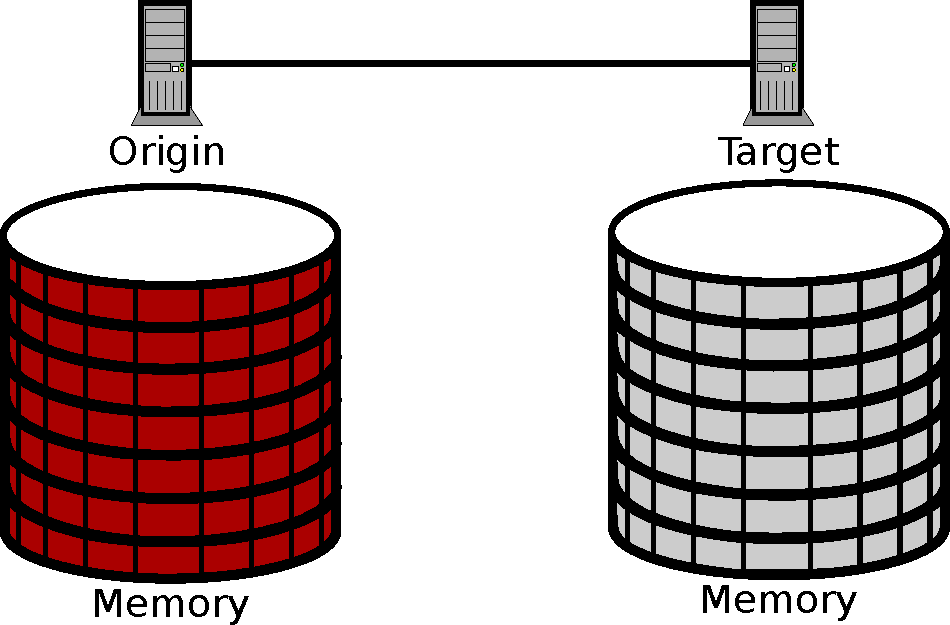
\includegraphics[width=0.7\linewidth]{images/nomad_stage1}
  \caption{NomadBIOS: 1. Migrationsphase}
  \label{fig:nomad_stage1}
\end{figure}
Der Speicher auf dem Ursprung, der dem Gastsystem gehört, wird
zunächst für Schreibzugriffe gesperrt und der Kopiervorgang auf den
neuen Host wird gestartet. Wenn währenddessen Speicher geschrieben
wird, wird ein Page-fault ausgelöst, und das NomadBIOS kann die
entsprechende Speicherseite erneut zum Kopieren markieren. Danach wird
die Seite als für das Gastsystem beschreibbar markiert und
geschrieben.

Nach einem ersten Kopierdurchlauf werden so eine Reihe von
Speicherseiten noch zum Kopieren markiert worden sein. Es ist nicht
klar ob diese Seiten vor oder nach der letzten Manipulation zum
Zielsystem kopiert wurden~\ref{fig:nomad_stage2}.
\begin{figure}[h]
  \centering
  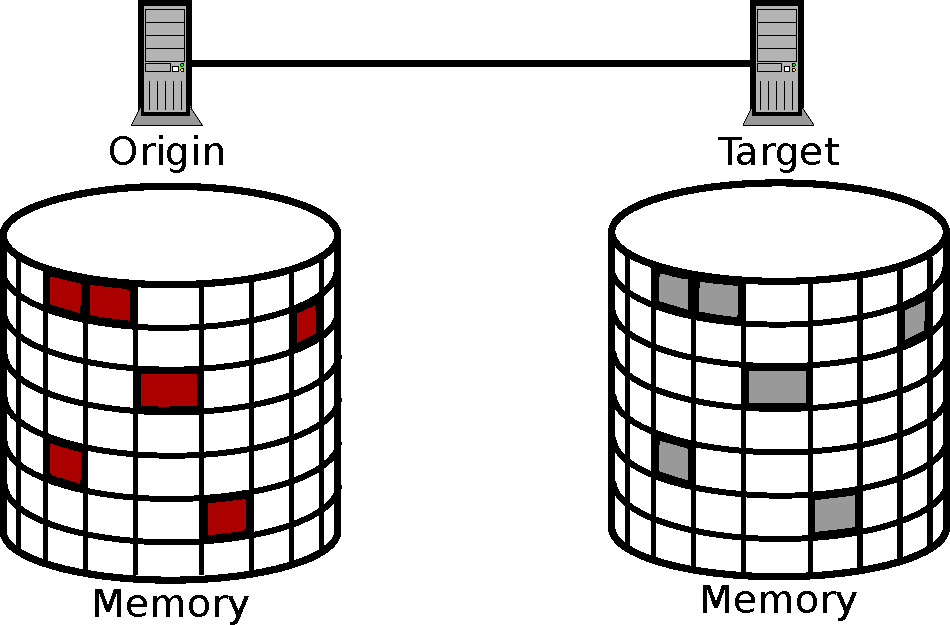
\includegraphics[width=0.7\linewidth]{images/nomad_stage2}
  \caption{NomadBIOS: 2. Migrationsphase}
  \label{fig:nomad_stage2}
\end{figure}
Diese können nun in einem weiteren, kürzeren Kopierdurchlauf mit dem
Zielsystem synchronisiert werden. Da dieser zweite Kopiervorgang
schneller vonstatten geht, werden währenddessen weniger Seiten wieder
vom Gastsystem beschrieben werden. Nach mehreren Iterationen ist das
Delta zwischen dem Gast und Zielsystem so weit geschrumpft, dass die
verbleibende Differenz in wenigen Millisekunden kopiert werden
kann. In diesem Moment wird der Gastprozess auf dem Ursprungssystem
eingefroren, die restlichen Seiten kopiert, und auf dem Zielsystem
gestartet\ref{fig:nomad_stage3}.
\begin{figure}[h]
  \centering
  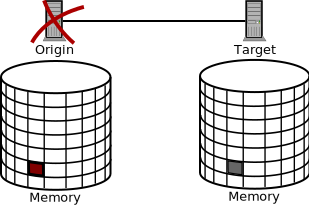
\includegraphics[width=0.7\linewidth]{images/nomad_stage3}
  \caption{NomadBIOS: 3. Migrationsphase}
  \label{fig:nomad_stage3}
\end{figure}
Wenn im gleichen Moment auch das Routing angepasst wird, so
kann die VM direkt weiterarbeiten, ohne das Benutzer mehr als einen
kurzen Latenzanstieg bemerken.

vMotion \ldots

\subsection{IBM}
Xen, active research to enable VM migration on a number of open-source
virtualization solutions (VirtualBox, KVM + Qemu)

\subsection{HP}
HP bietet Virtualisierungsdienste auf Basis von Microsoft's
\emph{HyperV}. \emph{HyperV} unterstützt in Windows Server 2008 R2
bereits Live-Migration von virtuellen Maschinen, der Migrationsprozess
läuft dabei analog zum NomadBIOS ab. Eine wesentliche Limitierung des
HyperV ist, dass alle physikalischen Maschinen Zugriff auf gemeinsamen
Speicher, z.B. Network-Attached-Storage oder ein Netzwerkdateisystem,
haben müssen, um VM Daten auszutauschen~\cite{hp2010hyperV}. Das kann
beim Umziehen zwischen geografisch entfernten Orten oft nicht
gewährleistet werden. HP hat hierfür sein \emph{Cluster Extension}
(CLX) Produkt erweitert. CLX ist zunächst eine Software zur
Replikation von Daten über große Distanzen. Mit den HyperV
spezifischen Erweiterungen kann CLX nun dazu genutzt werden, den
Zustand von VMs zwischen verschiedenen Rechenzentren zu
synchronisieren. Dabei ist CLX voll in den HyperV Live-Migration
Prozess integriert. Mit der CLX---HyperV Kombination kann
sichergestellt werden, das Replikation über Datencenter hinweg
VM-Migrationen unterstützt, und nicht behindert, indem während der
Migration dieser mehr Bandbreite zugestanden wird, damit die finale
Speicherseitensynchronisation (während der die Ursprungs-VM
eingefroren ist) so schnell wie möglich vonstatten geht. Wenn die
Migration abgeschlossen ist, macht CLX den neuen physikalischen
Standort der VM automatisch zum Master für die weitere Replikation.

Im März 2010 aktualisierte außerdem seine UNIX Distribution
\emph{HP-UX}. Teil dieses Updates war die Version 4.2 des hauseigenen
\emph{Integrity Virtual Machines} Hypervisors. Dieser enthält eine
\emph{Online Migration} Funktion, die ebenso mit CLX zusammen
eingesetzt werden kann~\cite{hp2010integrity}.

\subsection{Sun/Solaris}
Solaris Container

\subsection{Vergleich}
Vergleich der Eignung als Lösung für die oben genannten Probleme
zwischen dem von Dr. Jacob Gorm Hansen vorgestellen System und den Alternativen.


%%% Local Variables: 
%%% mode: latex
%%% TeX-master: "FelgentreffPape_2010_Live-MigrationInVirtuellenUmgebungen"
%%% End: 
